\section{Actividad No 03 –  Creating PL/SQL Blocks} 
		
\begin{enumerate}[1.]
	\item VOCABULARIO :
	\subitem Identify the vocabulary word for each definition below:
	\subitem-\_\_\_\_\_\_\_\_\_\_\_\_\_\_\_\_:Unnamed blocks of code not stored in the database and do not exist after they are executed
	\subitem-\_\_\_\_\_\_\_\_\_\_\_\_\_\_\_\_:A program that computes and returns a single value
	\subitem-\_\_\_\_\_\_\_\_\_\_\_\_\_\_\_\_:Named PL/SQL blocks that are stored in the database and can be declared as procedures or functions
	\subitem-\_\_\_\_\_\_\_\_\_\_\_\_\_\_\_\_:Software that checks and translates programs written in highlevel programming languages into binary code to execute
	\subitem-\_\_\_\_\_\_\_\_\_\_\_\_\_\_\_\_:A program that performs an action, but does not have to return a value

	\item Try It / Solve It
	\subitem 01- Complete the following chart defining the syntactical requirements for a PL/SQL block:

	\begin{center}
	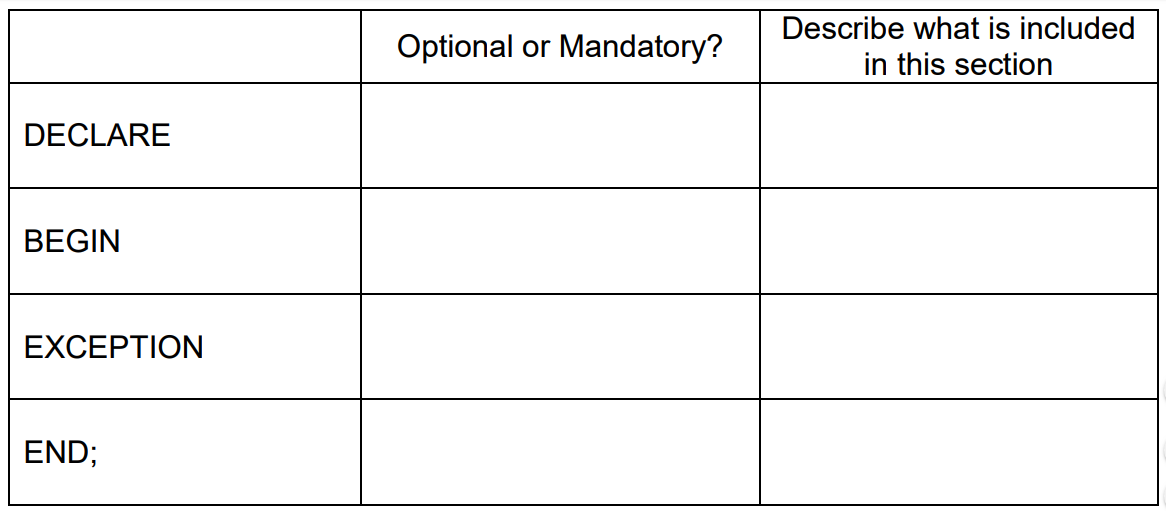
\includegraphics[width=15cm]{./Imagenes/actividad01}  
	\end{center}	
	\subitem 02- Which of the following PL/SQL blocks executes successfully? For the blocks that fail, explain why they fail
	\\
	\subitem A. BEGIN
	\subitem    END;
	\subitem B. DECLARE
 	\subitem    amount INTEGER(10);
	\subitem    END;
	\subitem C. DECLARE
	 \subitem   BEGIN
	 \subitem   END;
	\subitem D. DECLARE
	 \subitem	amount NUMBER(10);
	 \subitem	begin
	 \subitem	DBMS\_OUTPUT.PUT\_LINE(amount);
	 \subitem	END;
	
	\subitem 03- Fill in the blanks:
	\subitem A. PL/SQL blocks that have no names are called \_\_\_\_\_\_\_\_\_\_\_\_\_\_\_\_\_\_.
	\subitem B. \_\_\_\_\_\_\_\_\_\_\_\_\_\_\_ and \_\_\_\_\_\_\_\_\_\_\_\_\_\_\_ are named blocks and are stored in the database

	

\end{enumerate}

